\section{Set dati GuitarSet}
\textbf{tempo di lavoro:} \\
\newline
Fortunatamente, su Internet abbiamo trovato un \textit{data set} di file audio di chitarra già pronto su cui lavorare. Il \textit{GuitarSet}, chiamato così dal suo creatore, è costituito dai file audio e dai suoi \textbf{tab}.\\
Questo \textit{data set} contiene 360 estratti di canzoni della durata di circa 30 secondi l'uno. Essi sono il risultato delle seguenti combinazioni:
\begin{itemize}
	\item 6 persone suonano ciascuno gli stessi 30 fogli
	\item Vengono registrate 2 versioni diverse: comping e soloing
\end{itemize}
I 30 fogli sono generati da una combinazione di
\begin{itemize}
	\item \textbf{5 stili}: Rock, Cantautore, Bossa Nova, Jazz e Funk
	\item \textbf{3 progressioni}: 12 Bar Blues, Autumn Leaves e Pachelbel Canon.
	\item \textbf{2 Tempi}: lento e veloce.
\end{itemize}
Gli estratti sono registrati sia con il pickup esafonico che con un microfono a condensatore Neumann U-87.
Ci sono tre registrazioni audio per ogni estratto:
\begin{itemize}
	\item \textbf{hex}: file wav originale a 6 canali dal pickup esafonico;
	\item \textbf{hex\_cln}: file wav esadecimali con rimozione delle interferenze applicata;
	\item \textbf{mic}: registrazione monofonica dal microfono di riferimento
\end{itemize}
Noi abbiamo usato registrazioni di tipo \textbf{mic} perchè sono quelle che più si avvicinano al caso delle registrazioni tramite microfono dello smartphone.\\
\newline
Ciascuno dei 360 estratti ha anche un file .jams che memorizza 16 annotazioni da cui prenderemo le tab:
\begin{itemize}
	\item Intonazione:
	\begin{itemize}
		\item 6 annotazioni \textit{pitch\_contour} (1 per stringa);
		\item 6 annotazioni \textit{midi\_note} (1 per stringa);
	\end{itemize}
	\item Beat e tempo:
	\begin{itemize}
		\item 1 annotazione \textit{beat\_position};
		\item 1 annotazione del tempo;
	\end{itemize}
	\item Accordi:
	\begin{itemize}
		\item 2 annotazioni di accordi (istruite ed eseguite).
	\end{itemize}
\end{itemize}
Noi useremo le annotazioni \textit{midi\_note} che contengono le tab.
\subsection{Ricavare le tab dai file .jams}
Innanzitutto calcoliamo i \textit{frame} per ogni file audio, così da poter ricavare un immagine e la corrispondente tab per ogni frame.
Per calcolare l'istante di tempo per ogni frame utilizziamo la funzione \textit{get_times()}
\pythonexternal{./codes/times.py}

Successivamente calcoliamo 
\pythonexternal{./codes/labels.py}


\textit{NumPy} è una libreria che aggiunge supporto a grandi matrici e array multidimensionali insieme a una vasta collezione di funzioni matematiche di alto livello per poter operare efficientemente su queste strutture dati.\\
\newline
I dati sono stati compressi in \textit{numpy array} (.npz) per organizzarli meglio altrimenti avremmo avuto un'immagine e una label per ogni file audio.

\pythonexternal{./codes/labels.py}

\subsection{Trasformata a Q Costante in Librosa}
\textit{Librosa} è una libreria per la musica e l'analisi audio. Fornisce gli elementi costitutivi necessari per creare sistemi di recupero delle informazioni musicali.\\
\newline
La trasformazione a Q Costante può essere facilmente applicata ai file audio utilizzando la libreria \textit{librosa}.

\pythonexternal{./codes/librosa.py}
Ogni file audio è stato diviso ogni tot secondi in modo da stampare le note che sono state suonate sulla chitarra sempre tramite la libreria \textit{librosa}. L'obiettivo è quello di prendere l'immagine appena ottenuta e di darla in input alla rete CNN. Sperimentalmente, abbiamo visto che per ottenere un buon valore di accuratezza nella rete, le immagini devono essere stampate ogni 0.2 secondi.

\begin{figure}[H]
	\centering
	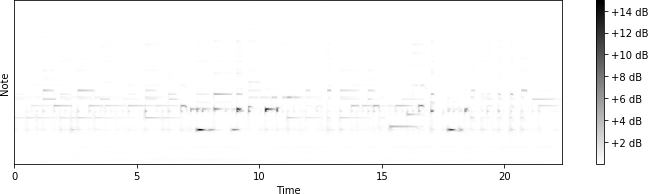
\includegraphics[scale=0.90]{./images/img7.png}
\end{figure}
Se il tempo fosse stato inferiore avremmo avuto immagini di file audio con solo note singole e quando la rete avrebbe dovuto riconoscere più note non sarebbe stata in grado di farlo. Nell'immagine seguente è possibile vedere che le lettere sulle note si ripetono. Ad esempio, la lettera F si trova sulla corda F e D. Se la mano è posizionata sulla corda A, è impossibile che si riesca a suonare la F della nota G. Dunque, un istante di tempo troppo corto non aiutava la rete a riconoscere la nota giusta.

\begin{figure}[H]
	\centering
	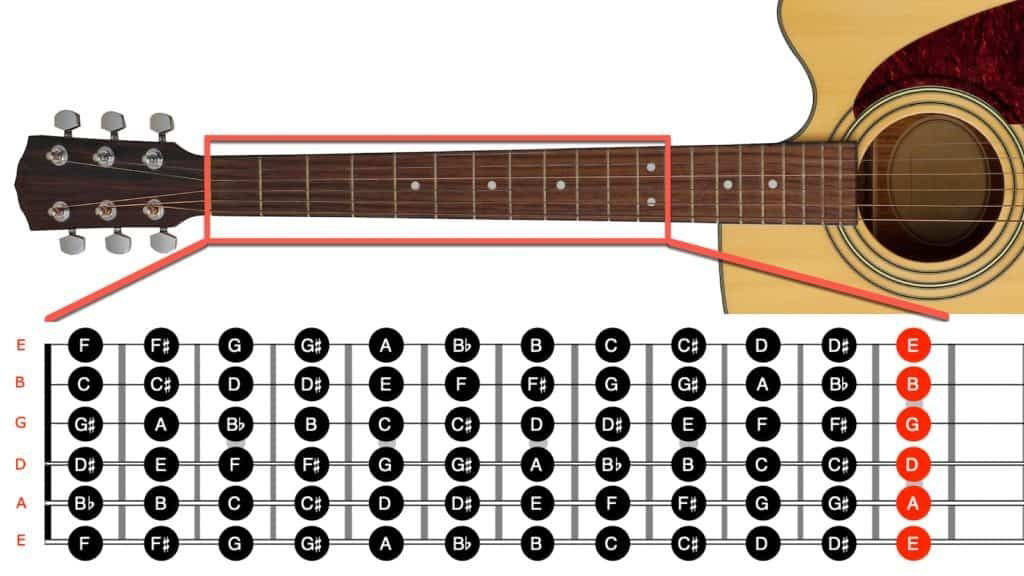
\includegraphics[scale=0.20]{./images/img12.jpg}
\end{figure}

L'immagine risultante da \textit{librosa} ha dimensione 192x9.\\

%da spostare
I tab sono matrici 6x19 e hanno caratteristica di essere \textit{one-shot} cioè si può trovare un uno solo in ogni riga. Ad ogni uno presente nella riga corrisponde a un nota. Le sei righe della matrice corrispondono alle sei note della chitarra mentre i tasti sono diciotto. La colonna in più, più precisamente la prima, indica che nella prima colonna la corda non è stata toccata.

\subsection{Pre-elaborare i dati}

% keras e
	% https://www.pyimagesearch.com/2019/10/21/keras-vs-tf-keras-whats-the-difference-in-tensorflow-2-0/

\section{Modello della rete}
\textbf{tempo di lavoro:} \\
\newline
\subsection{Uso di Keras}
Keras consente di implementazione algoritmi basati su reti neurali. Permette di sviluppare e prototipare in maniera semplice e veloce modelli nell’ambito del machine learning e del deep learning.\\
\pythonexternal{./codes/norm2.py}

\pythonexternal{./codes/modello.py}
\subsection{Compilazione del modello}
\textbf{tempo di lavoro:} \\
\newline
\pythonexternal{./codes/compilare.py}
\subsection{Addestramento del modello}
\textbf{tempo di lavoro:} \\
\newline
Dopo diverse prove sperimentali, abbiamo deciso di eseguire il modello per 30 epoche:

Questo modello raggiunge una precisione di circa 0,91 (o 91\%) sui dati di addestramento.
\begin{figure}[H]
	\centering
	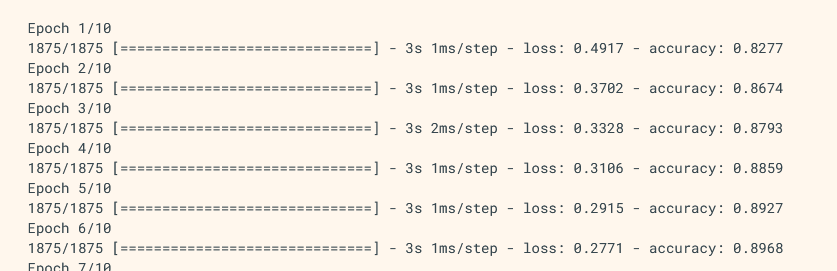
\includegraphics[scale=0.70]{./images/img5.png}
\end{figure}

\section{Accuratezza del modello}
\textbf{tempo di lavoro:} \\
\newline
Abbiamo confrontato le prestazioni del modello sul set di dati di test:

\pythonexternal{./codes/accuratezza.py}
\begin{figure}[H]
	\centering
	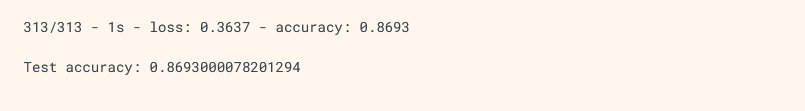
\includegraphics[scale=0.70]{./images/img6.png}
\end{figure}